\oldpage{406}its place, and to my great delight it stopped the hemorrhage almost
instantly. The remainder of the blood which was in the vessel I took
through the same process and reduced it to a fine powder for future use.

\textsc{Remarks}.---The use of blood as a remedial agent is not new to the
profession as a reference to the \ThisJournal{Journal}, page 299 will show, where
Dr.\ Miller refers to the use made of it by Mauthner in ansemia, as
referred to by Dr.\ Davis, of Illinois, in the Transactions of the Illinois
State Medical Society for 1852, who says it may be given when inspissated
in doses of from ten to sixty grains at a dose, or dissolved in
water. The therapeutic use of blood is also referred to in the \booktitle{Am.\ Med.\ Journal}
for 1853 and perhaps in other periodicals. But none of
these refer to the \emph{styptic} properties it is supposed to possess by Dr.\ Van
Buskirk, and which one single experiment neither proves or disproves.
The Pencil Savans are accustomed to deny nothing until it is
thoroughly disproved, and to admit nothing until it is thoroughly established,
but rather to \emph{receive} the opinions of others and await farther
and full proof before their final disposition, and in this regard we may
do well to follow their example.\hfill{}C.

\begin{figure}[H]
  \centering
  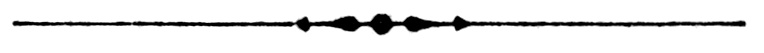
\includegraphics{pages/illustrations/arrow_bullet_divider.jpg}
\end{figure}

\section*{Notes and Observations.}

\byline*{\ProperName{T.~C.\ Miller}, \md}

\SectionStartWords{Ammonia Valerianicum} [\emph{Valerianate of Ammonia}]. This is formed
by the saturation of the Valerianic acid with the carbonate of ammonia.
It is usually a fluid, although an imperfect crystallization has been obtained
of the salt. In warm weather even the crystals are apt to deliquesce
into a syrupy fluid, having a strong valerianic odor, and a
slight odor of ammonia.

\ProperName{Ottinger} of Munich, Germany, has highly recommended this preparation
in Asiatic Cholera in the following form.

\begin{center}
\begin{tabbing}
  \prescription. \= Ammonia Valerianici, \scruple j. \\
    \> Aqua Destillat., f \ounce iij. \\
    \> Syrup. Sacch., f \ounce ss.
\end{tabbing}
\end{center}

M.\quad{}Dose, one tablespoonful once in from 15 to 30 minutes.

\ProperName{Ottinger} used this mixture to the exclusion of every other internal
remedy, and after the severity of the attack had passed and reaction
was established, he gave but from four to six doses daily. He also
ordered ice to be rubbed over the abdomen externally, occasionally
changing the cold water for hot or placing the patient in a hot bath in\endinput
